%%%%%%%%%%%%%%%%%%%%%%%%%%%%%%%%%%%%%%%%%%%%%%%%%%%%%%%%%%%%%%%%%%%%%%%
%%%%%%%%%%%%%%%%%%%%%%%%%%%%%%%%%%%%%%%%%%%%%%%%%%%%%%%%%%%%%%%%%%%%%%%
%%%%%                                                                 %
%%%%%     <file_name>.tex                                             %
%%%%%                                                                 %
%%%%% Author:      <author>                                           %
%%%%% Created:     <date>                                             %
%%%%% Description: <description>                                      %
%%%%%                                                                 %
%%%%%%%%%%%%%%%%%%%%%%%%%%%%%%%%%%%%%%%%%%%%%%%%%%%%%%%%%%%%%%%%%%%%%%%
%%%%%%%%%%%%%%%%%%%%%%%%%%%%%%%%%%%%%%%%%%%%%%%%%%%%%%%%%%%%%%%%%%%%%%%

\chapter{Task Description}
Include the task description \textbf{pdf} you got from your
assistant(s) with the \shell{\textbackslash includepdf} command.
% include the task description pdf!
%\includepdf[pages=-, turn=false, scale=0.9]{../../task/TaskDescription.pdf}


\chapter{Declaration of Originality}\label{chap:originality}
Include the declaration of authorship with the \shell{\textbackslash
  includepdf} command (sign it and scan it). For more information
about plagiarism, please visit
\url{https://www.ethz.ch/students/en/studies/performance-assessments/plagiarism.html}

\begin{itemize}
\item \textbf{English version:}
  \url{https://www.ethz.ch/content/dam/ethz/main/education/rechtliches-abschluesse/leistungskontrollen/declaration-originality.pdf}
\item \textbf{German version:}
  \url{https://www.ethz.ch/content/dam/ethz/main/education/rechtliches-abschluesse/leistungskontrollen/plagiat-eigenstaendigkeitserklaerung.pdf}
\end{itemize}

% include the signed declaration of authorship!
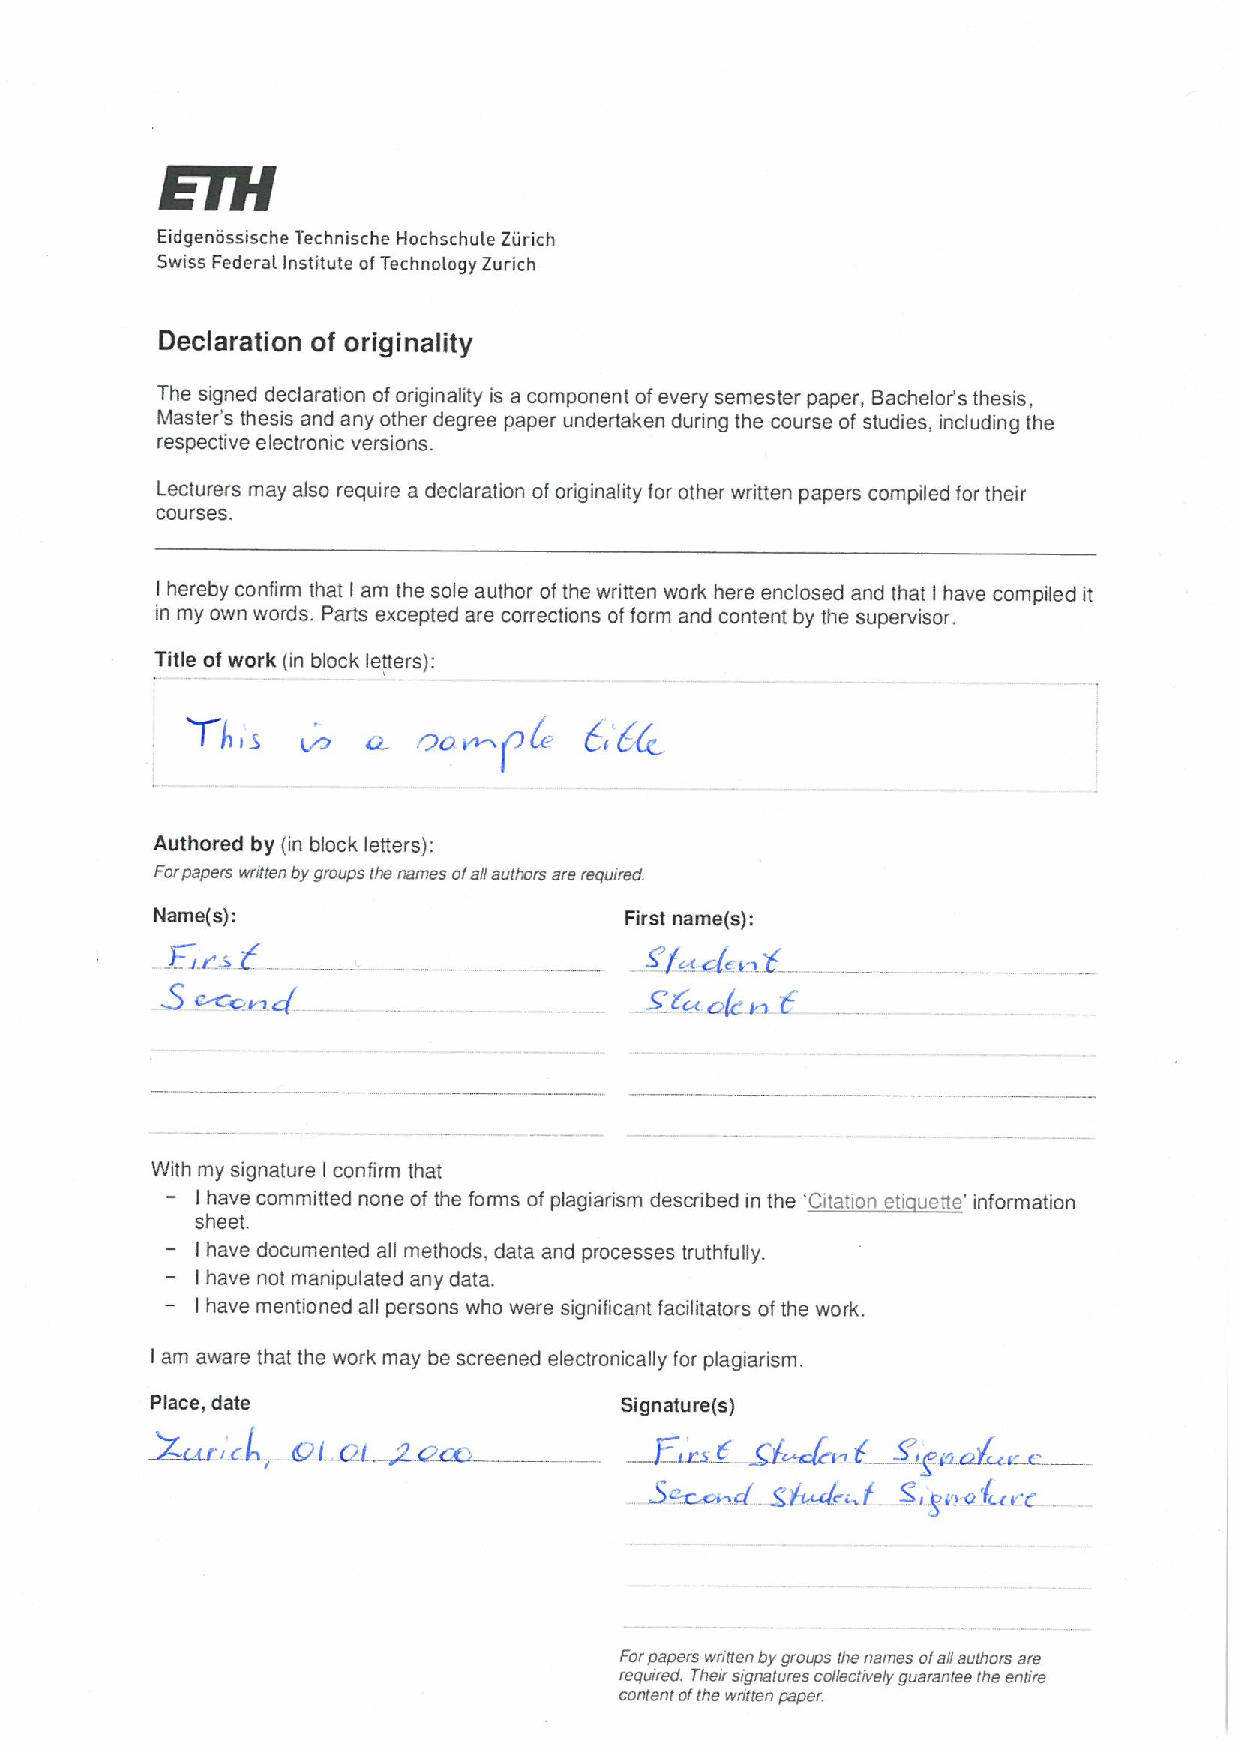
\includepdf[pages=-, turn=false, scale=0.9]{./figures/declaration_of_originality}


\chapter{File Structure}
Describe how the project directories/files are organized, e.g.:

\begin{flushleft}
\dirtree{%
.1 /.
  .2 README \DTcomment{A README with some general information about the project.}.
  .2 01\_report \DTcomment{The source files of the project report.}.
  .2 02\_presentation \DTcomment{The source files of the presentation.}.
  .2 03\_designflow \DTcomment{Some designflow-specific files.}.
}
\end{flushleft}

What needs to be done to run an RTL simulation (stimuli generation,
compilation...)?


\chapter{Datasets}
If you have a data set comprising several test images, you could
depict and describe them here. Use a simple naming scheme such that
you can easily refer to certain elements of this data set in the text.


\chapter{More Evaluation Results}
If you conducted an extensive evaluation you could move surplus
graphs/results to the appendix.


\chapter{Algorithms / Tables}
Large algorithm boxes and tables may clutter your chapters and impair
the readability. If they are not very important, consider moving them
to the appendix as well.


\chapter{ASIC Datasheet ($<$Chipname$>$)}

If you have designed an \gls{asic} during your work, you should
include a datasheet for your chip into the report. As soon as you
start testing your fabricated chip, you will be glad to have such a
datasheet. An example structure of such a datasheet is given in the
following. For more inspirations on what you may include in your
datasheet, have a look at the datasheet of a commercial \gls{ic}.

\minitoc

\section{Features}
\begin{itemize}
\item Lorem ipsum dolor sit amet, ...
\item Lorem ipsum dolor sit amet, ...
\item Lorem ipsum dolor sit amet, ...
\item Lorem ipsum dolor sit amet, ...
\end{itemize}

\section{Applications}
\lipsum[2]

\section{Description}
\lipsum[2]

\section{Packaging}
\lipsum[2]

\section{Bonding Diagram}
\lipsum[2]

\begin{figure}[htbp]
  \centering 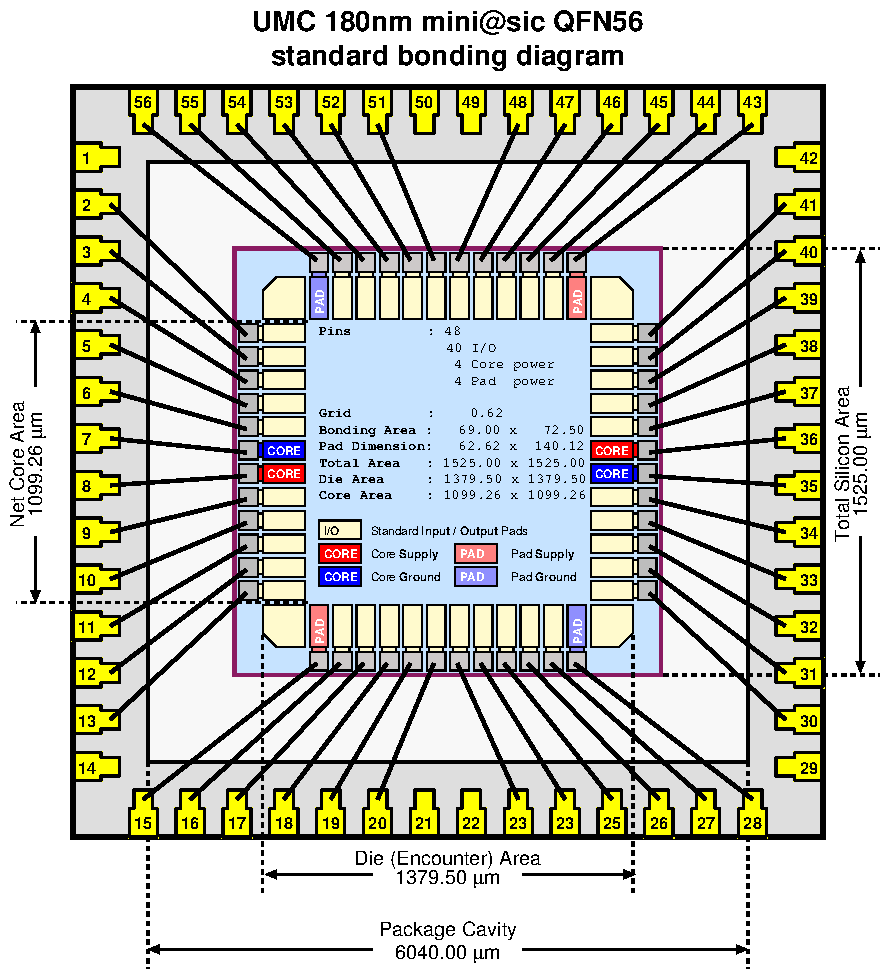
\includegraphics[width=0.9\textwidth]{./figures/qfn56_180_std}
  \caption{Bonding diagram.}
\end{figure}

\section{Pin Map}
\lipsum[2]

\begin{figure}[htbp]
  \centering 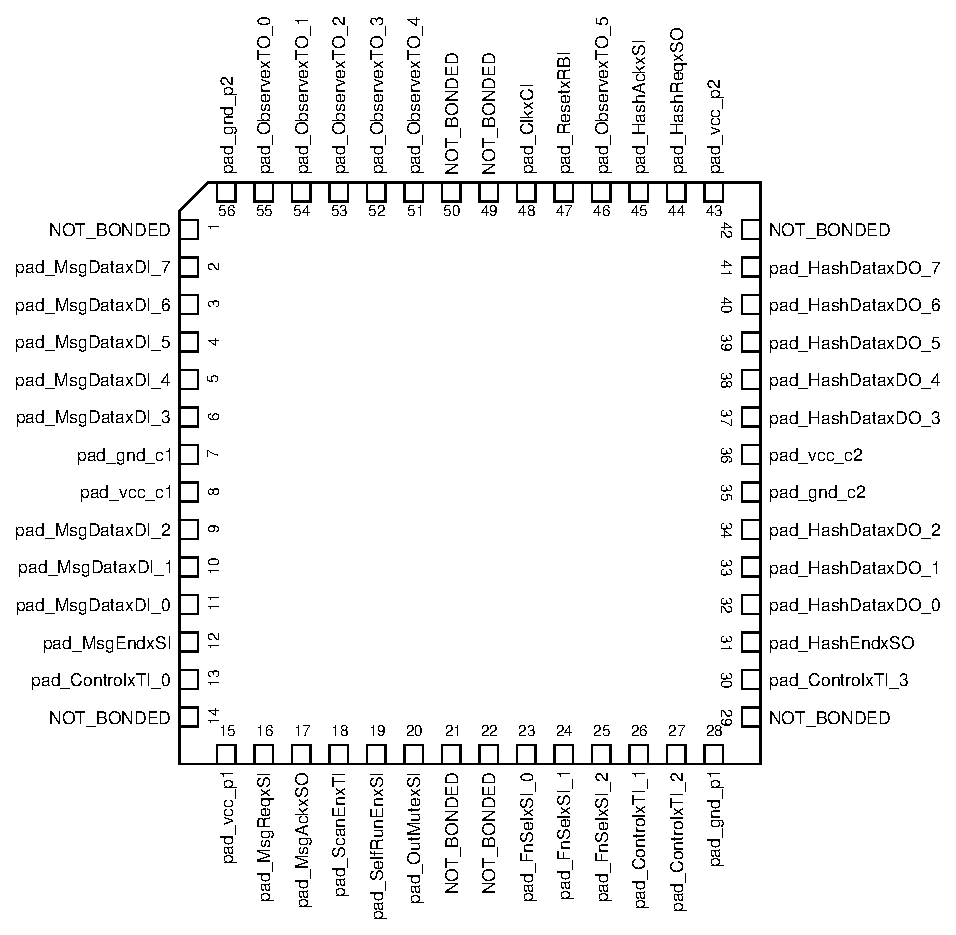
\includegraphics[width=1.0\textwidth]{./figures/asic_pinout}
  \caption{$<$Chipname$>$ pinout.}
\end{figure}

\section{Pin Description}
\lipsum[2]

\section{Interface Description}
\lipsum[2]

\section{Register Map}
\lipsum[2]

\section{Operation Modes}
\lipsum[2]

\subsection{Functional Modes}
\subsection{Test Modes}

\section{Electrical Specifications}
\lipsum[2]
\subsection{Recommended Operating Regions}
\subsection{Absolute Maximum Ratings}
